\chapter{Discussion}
\label{chapter:discussion}

\section{Interpreting the WER results}
Our experiments show the different methods to accelerate all the different parts of the pipeline for training ASR models for data scalability. We now report the word error rate, word error rate with punctuations and capitalizations considered and the character error rate among the three different methodologies. The first method is the centralized training with a single GPU with multiprocessing used only for data loading and preprocessing. The second methodology is the Distributed Data Parallel method, which is the synchronous training using 4 GPUs, with one process on each GPU for training. The third method is the asynchronous training with Hogwild, with 3 processes using a single GPU to share weights and update them in parallel. These results are reported in Table \ref{table:overall_wer}. but to compare the training methods for large-scale datasets and to showcase the best workflow for such experiments, we now compare the different metrics for the largest training dataset size, i.e. 20,000 hours. 
\begin{table}[ht]
\centering
\begin{tabular}{c | c c c | c }
\hline
     & WER & WER-P & CER-P & Training Wall-time (hrs)\\
 \hline
  1-GPU & 14.01\% & 17.12\% & 7.67\% & \textbf{59} \\
  4-GPU DDP & 10.87\% & 13.69\% & 5.73\% & \textbf{32} \\
  1-GPU Hogwild & 24.09\% & 27.56\% & 13.81\% & \textbf{NA} \\
 \hline
\end{tabular}
\caption{\label{table:overall_wer} WER, WER-P and CER-P comparison for single GPU, single GPU, multi GPU \acrshort{ddp}, 1-GPU Hogwild runs for the 20,000 training hours dataset. The table also shows the wall clock time to convergence with the different setups.}
\end{table}

The synchronous \acrshort{ddp} training job with \acrshort{wer} of 10.87\% and \acrshort{cer}-P of 5.73\% is the best result obtained overall. Synchronous training methods work well when the different \acrshort{gpu}s are similar in their processing power and memory storage. This avoids stragglers and training synchronization can happen smoothly. This can also be seen in our experiments that the time to convergence is reduced by half with the use of \acrshort{ddp} on multiple GPUs. 

Some caution has to be taken before reading these results, because the hyperparameters were optimized only once at the beginning of the experiments, and it is possible that for the different methods, varying the hyperparameters could lead to better results. The main aim of this thesis was not to get the best \acrshort{wer} for the dataset but to evaluate the best practices and methods for data scalability, and hence this step was not given much prominence during the experiments. 

\section{Evaluation with LibriSpeech}
Since the dataset size is big, we wanted to evaluate the model's generalization capabilities. We employ similar strategy as the researchers of the People's Speech Dataset \cite{Galvez2021TheUsage}. We evaluate our best model on the LibriSpeech\cite{Panayotov2015Librispeech:Books} test datasets without any transfer learning, so the LibriSpeech data is completely unseen data for the model. Table \ref{table:libri} shows the test word error rates for LibriSpeech datasets and compare it with the People's Speech Dataset results. Since LibriSpeech data does not contain any punctuations and capitalization, we normalize the hypothesis text from our model before calculating the \acrshort{wer} metrics. 

\begin{table}[ht]
\centering
\begin{tabular}{c | c c | c c }
\hline
\textbf{Results} & \multicolumn{2}{c|}{\textbf{test-clean}} & \multicolumn{2}{c}{\textbf{test-other}}\\\cline{2-5}
    & WER & CER & WER & CER\\
 \hline
  Our Model & 22.46\% & 10.62\% & 37.93\% & 20.41\%\\
  People's Speech \cite{Galvez2021TheUsage} & 32.17\% & 18.86\% & 57.56\% & 41.2\% \\
 \hline
\end{tabular}
\caption{\label{table:libri} WER and CER comparison for test-clean and test-other datasets with the People's Speech model}
\end{table}

Although, the results with our model are worse than state-of-the-art models on LibriSpeech, we manage to outscore the people's speech models by 30\% on the test-clean dataset and by 35\% on the test-other dataset which shows the model can generalize pretty well.

\section{Effect of accent on the WER}
In Section \ref{section:bizspeech}, we had discussed the challenges in the dataset concerning the utterances which are spoken by people from different parts of the world, including non-native speakers of English, which is particularly interesting and useful for building a diverse model. We compare the word error rates for our best model with Google's Azure's results and also analyse the drop in accuracy between native and non-native utterances in Figure \ref{fig:wer_cloud_final} 

\begin{figure}[ht]
  \begin{center}
    % below the size of the figure has been reduced for example
    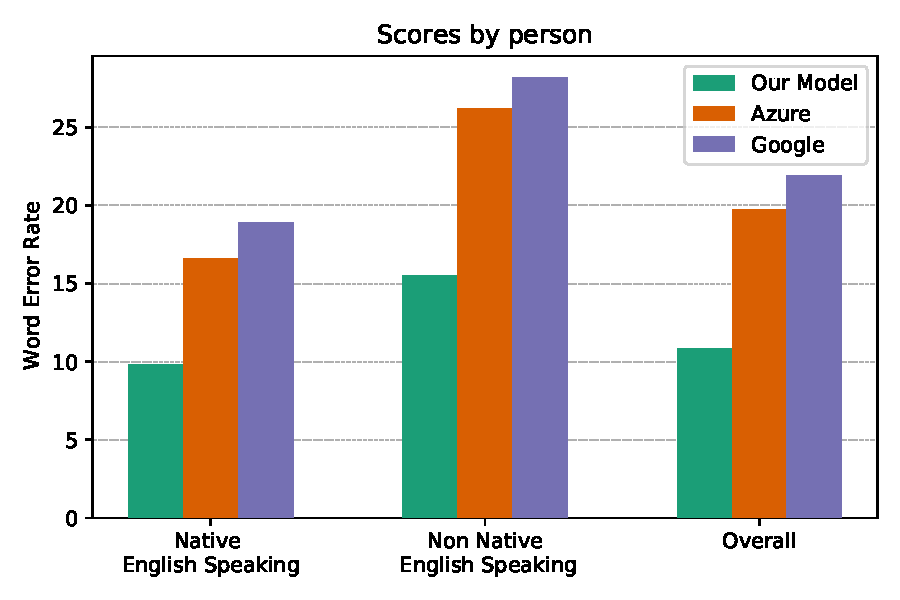
\includegraphics[width=\textwidth]{images/wer_cloud_final.pdf} 
    \caption{Word error rates comparison for native and non-native speakers of English between Google, Azure and our models.}
    \label{fig:wer_cloud_final}
  \end{center}
\end{figure}

The word error rates for the native and non-native speakers are calculated on different utterances for our model. This is due to overlap between the utterances used for cloud services to estimate \acrshort{wer} and the training set of our model. There is a consistent degradation of performance pertaining to non-native English speakers. 

%spgispeech results

\section{Future Work}

\subsection{Dataset related work}
The dataset used is large and this has enabled all the experiments that we have conducted, but the dataset is not without its drawbacks and future work can be done to address some of these inconsistencies. There are phrases like "Operator Instructions" which are discussed in Section \ref{section:bizspeech} which are wrong transcriptions of what is being said in the audio, and this only came to our attention in the later stages of our experiments. Although some preprocessing steps were taken, the dataset needs more thorough cleaning to remove utterances like the above example from the dataset, which can then lead to better models.

The dataset can also be used for a wide variety of other applications like named entity recognition when properly tagged and in other domains to infer business related results based on the speech in the earnings calls. Also, due to the varied nature of the speakers, it can also be filtered and used to train models which are designed to work with a diverse set of speakers.  

\subsection{Future Experiments}
Changing the model architecture can be tried and experiments involving scaling both model and data can be analysed and the correlation between the two scaling methods can be studied in detail. This could help establish a practical formula which can help researchers decide what minimum amount of data will be required to train models with certain number of parameters. 

With more time, we would have liked to tune hyperparameters for each type of training and analyse the best word error rates from the different techniques. Currently, the results indicate that methods that work with large batch sizes have fared well and models seem to struggle when batch size is reduced. It will be interesting to see if this holds even after varying the other hyperparameters like the learning rate, adding a learning rate scheduler, different optimizers etc. In all our experiments, the acoustic models are trained end-to-end with punctuations, capitalizations and other special characters. This is one of the biggest unknown in the experiments, about how the model would vary if it was trained with the normalized text instead. 

\subsection{Evaluation Methods}
For evaluating the models, we choose the best validation word error rate checkpoint as the final model to be used with the test set. However, in many cases we observed a sharp decline between the validation word error rates and the test word error rates even when both the sets are unseen and sampled randomly. This can be avoided by techniques like averaging checkpoints over multiple epochs, which have competitive error rates. This method should be used in the future experiments.